
\section{Software description}

\textit{Describe the software. Provide enough detail to help the reader understand its impact. }

\subsection{Software architecture}

Oprogramowanie \SoftwareName wykorzystuje platformę programistyczną Matlab/Octave oraz silnik gier Unity. Część przeznaczona  dla silnika gier jest napisana w języku C\verb|#|. Implementuje mechanikę rozgrywki w grę typu tower defense. Rolę gracza pełni oprogramowanie napisane w języku Matlab. Komunikacja między oprogramowaniem w Matlab-ie a grą odbywa się na zasadzie kilent-serwer  (fig.~\ref{Fig:architecture}). Gra oczekuje na polecenia nasłuchując na wybranym porcie. Możliwa jest komunikacja zdalna poprzez internet. Oprogramowanie w Matlab-ie  jest zbiorem funkcji pozwalających na realizację badań metod decyzyjnych. Umożliwia pobieranie od gry aktualnych informacje o jej stanie i pozwala na  przekazywanie jej komend sterujących realizujących akcje stawianie nowych wież na planszy oraz wypuszczania nowych przeciwników. 

\begin{figure}
\begin{tikzpicture}
\node[rectangle,draw,minimum width = 3.5cm,minimum height = 1.5cm,label=above:{Player}] (r) at (-2.5,4.5) {Matlab/Octave};
\node[anchor=center,inner sep=0,label=above:{Game}] (game) at (4,4.5) {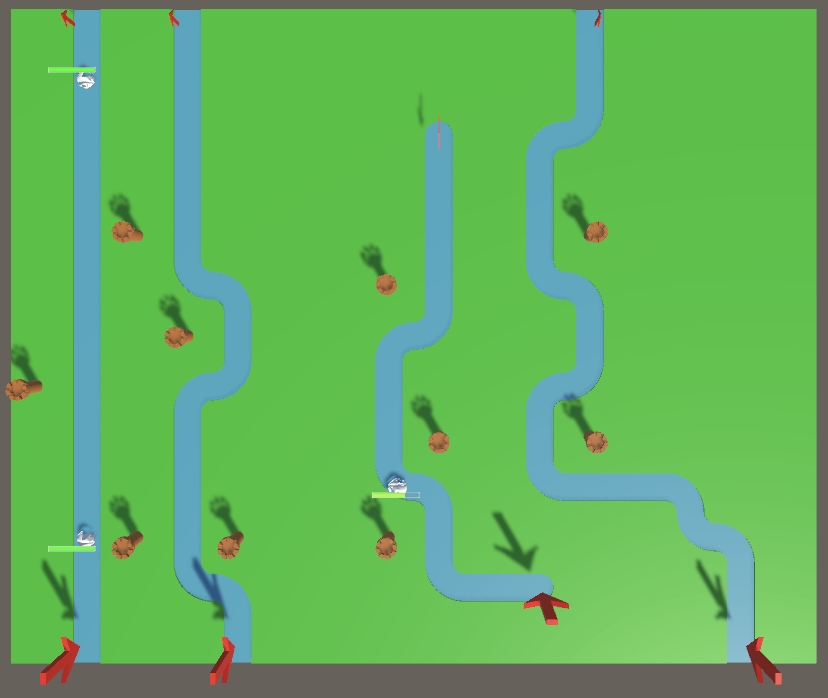
\includegraphics[width=3cm]{images/game.png}} ;
\node[anchor=center,inner sep=0, label=below:{Reports}] (tabaular) at (-2.5,1) {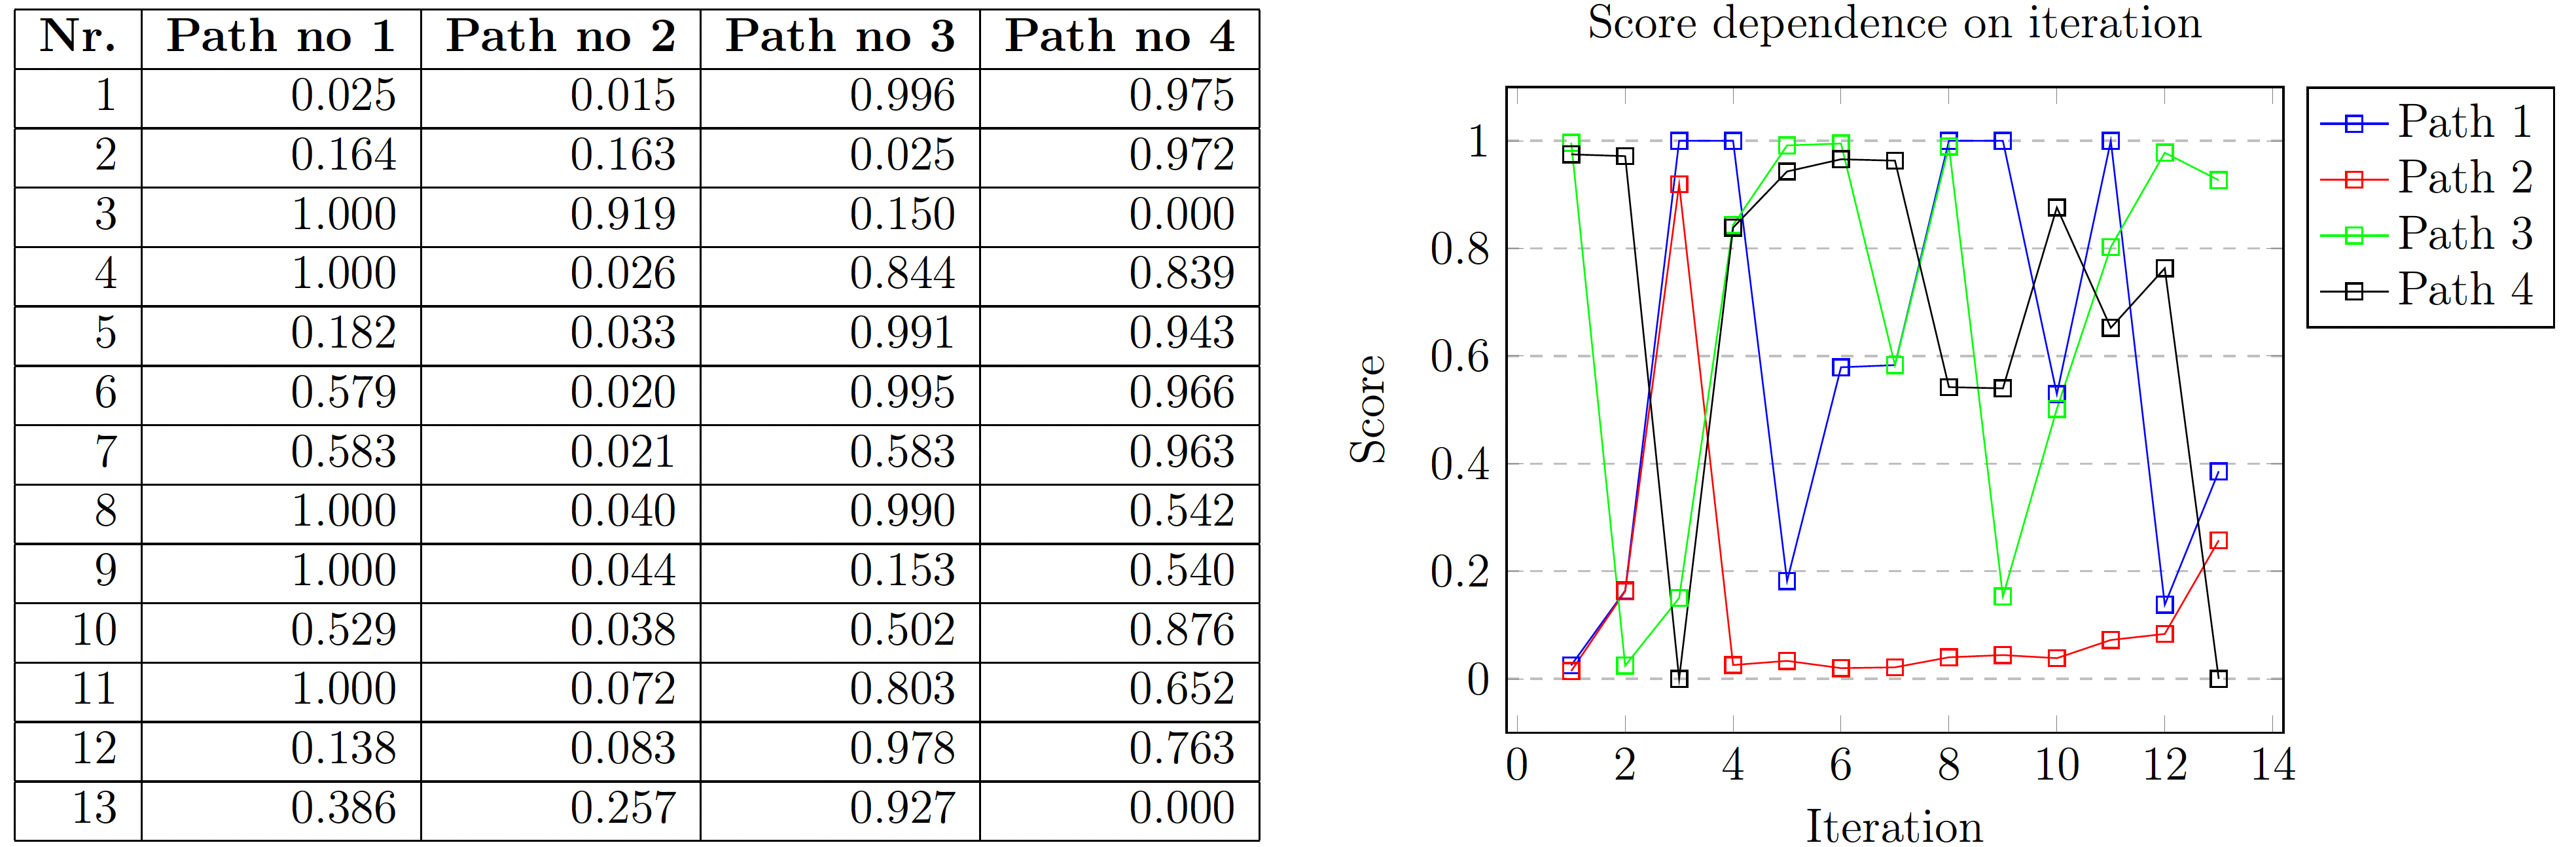
\includegraphics[height=2.5cm]{images/latexReports.png}};
\draw[oneArrowinverseStyle] (r.east) + (0,-0.1) -- ++(3.3,-0.1) node[midway,below]{Answer};
\draw[oneArrowStyle] (r.east) + (0,0.1) -- ++(3.3,0.1) node[midway,above]{Command};
\draw[oneArrowStyle] (r) -- (tabaular);

\end{tikzpicture}

\caption{Architektura systemu}
\label{Fig:architecture}
\end{figure}

Rysunek~\ref{Fig:softwareArchitecture} przedstawia ważniejsze moduły gry tower defense. Jednym z najważniejszych jej elementów jest komponent UnityServer realizujący wymianę informacji w formacie XML z oprogramowaniem działającym na platformie programistycznej Matlab. Moduł ten dekoduje otrzymane rozkazy i w zależności od potrzeb komunikuje się z innymi komponentami przekazując im zadania i zbierając potrzebne dane. Komponent ManagementTilemap zajmuje się zarządzaniem najmniejszymi elementami mapy -- tile. Zleca komponentowi CreateTilemap wykonanie tilemap w oparciu o dostępne tile. Gromadzi informacje statystyczne związane z wydarzeniami na kafelkach takich jak przejście  przeciwnika, zabicie przeciwnika itp. Przechowuje informacje o różnych typach tile, a w tym o ich wyglądzie (ma dostęp do ich modeli 3D). Zleca komponentowi ManagementCost wyznaczenie optymalnej trasy ruchu minimalizującej koszt przejścia od punktu startowego do końcowego. Komponent Towers przechowuje informacje o wieży, jej parametrach oraz wyglądzie. Podobnie komponent EnemyInfo przechowuje informacje o przeciwniku, jego parametrach oraz wyglądzie. Komponent ManagementCash zajmuje się zarządzaniem cash. Wyznacza ile cash mają wieże ile przeciwnicy i jest odpowiedzialny za prezentowanie tej informacji na HUD-ie i jej aktualizację.  

\begin{figure}
\begin{tikzpicture}
\begin{class}{ManagementTilemap}{-8,20.5}
\end{class}
\begin{class}{CreateTilemap}{-2,20.5}
\end{class}
\begin{class}{UnityServer}{-5,17}
\end{class}
\begin{class}{ManagementCash}{0,13.5}
\end{class}
\begin{class}{Towers}{0,18.4}
\end{class}
\begin{class}{EnemyInfo}{(-1,9}
\end{class}
\begin{class}{ManagementCost}{(-7,6}
\end{class}

\unidirectionalAssociation{ManagementTilemap}{}{}{CreateTilemap}{}{}
\unidirectionalAssociation{ManagementTilemap}{}{}{ManagementCost}{}{}
\unidirectionalAssociation{UnityServer}{}{}{ManagementCost}{}{}
\unidirectionalAssociation{UnityServer}{}{}{ManagementCash}{}{}
\unidirectionalAssociation{UnityServer}{}{}{EnemyInfo}{}{}
\unidirectionalAssociation{UnityServer}{}{}{ManagementTilemap}{}{}
\unidirectionalAssociation{UnityServer}{}{}{Towers}{}{}
\unidirectionalAssociation{Towers}{}{}{CreateTilemap}{}{}
\unidirectionalAssociation{Towers}{}{}{ManagementCash}{}{}
\unidirectionalAssociation{EnemyInfo}{}{}{ManagementCash}{}{}

\node[anchor=center,inner sep=0,label=below:{Tower}] (towerCharacter) at (-10,9) {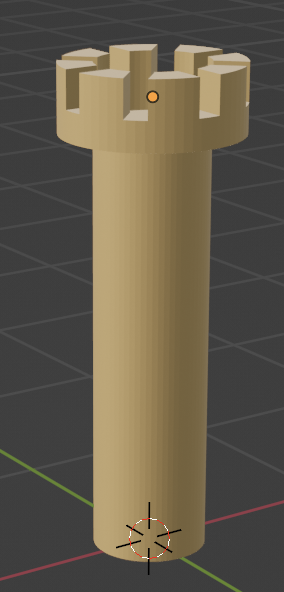
\includegraphics[height=2.5cm]{images/towerCharacter.png}};
\node[anchor=center,inner sep=0,label=below:{Enemy}] (enemyCharacter) at (-10,15.5) {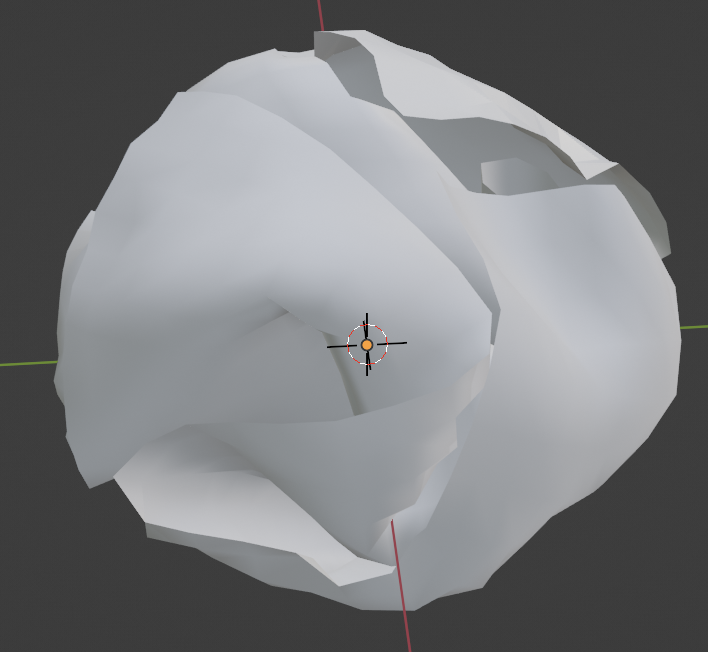
\includegraphics[height=2cm]{images/enemyCharacter.png}};
\node[anchor=center,inner sep=0,label=below:{Tile}] (tileCharacter1) at (-10,18) {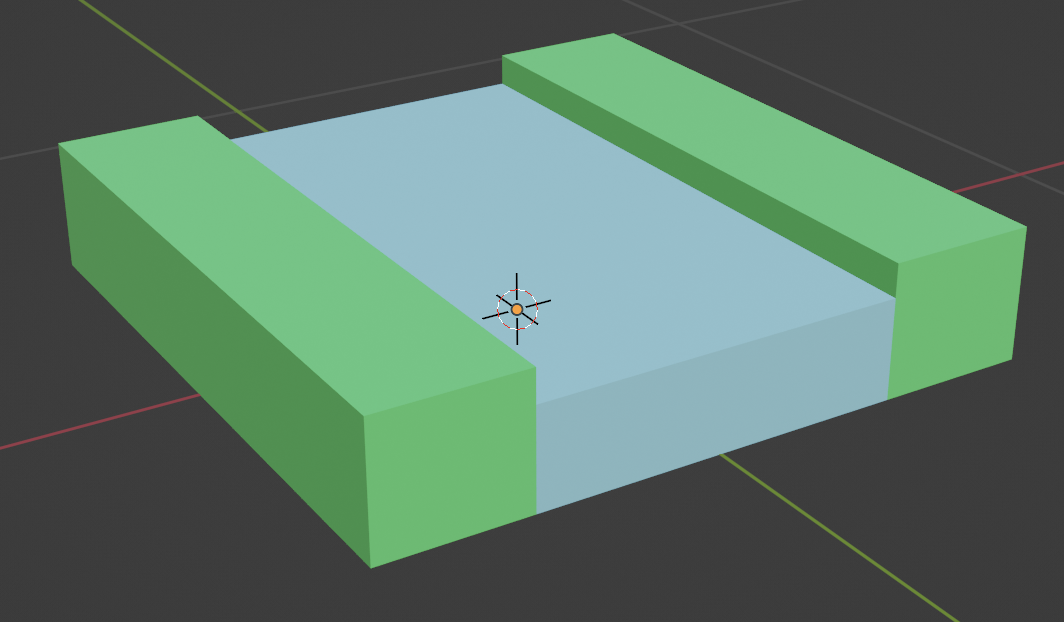
\includegraphics[height=1.5cm]{images/tileCharacter1.png}};
\node[anchor=center,inner sep=0,label=below:{HUD}] (HUD) at (-10,12.5) {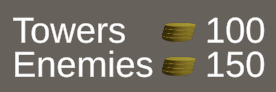
\includegraphics[height=1cm]{images/HUD.png}};

\draw[oneArrowStyle] (UnityServer) -- (towerCharacter);
\draw[oneArrowStyle] (UnityServer) -- (enemyCharacter);
\draw[oneArrowStyle] (ManagementCost) -- (towerCharacter);
\draw[oneArrowStyle] (EnemyInfo) -- (enemyCharacter);
\draw[oneArrowStyle] (Towers) -- (towerCharacter);
\draw[oneArrowStyle] (ManagementCash) -- (HUD);
\draw[oneArrowStyle] (ManagementTilemap) -- (tileCharacter1);


\end{tikzpicture}

\caption{Software architecture}
\label{Fig:softwareArchitecture}
\end{figure}



\textit{  Give a short overview of the overall software architecture; provide a pictorial overview where possible; for example, an image showing the components. If necessary, provide implementation details.}

 \subsection{Software functionalities}
\textit{  Present the major functionalities of the software.}

 \subsection{Sample code snippets analysis (optional)}
